\chapter{L2MuonSAにおけるNSWを用いた横運動量再構成アルゴリズムの動作検証と改良}\label{chapter5}
%本章ではNSWを用いたL2MuonSA部分飛跡再構成アルゴリズムについて、Run-3実データを用いた性能評価の結果について述べ、さらに検討したヒット選択アルゴリズムの説明および性能評価について述べる。


本章では、まず先行研究([\cite{article:kumaoka}, \cite{article:noguchi}])において開発、改良されたNSW部分飛跡再構成アルゴリズムについて紹介し、実データでの性能を評価した結果について述べる。
その後に、今回新しく検討したNSWヒット選択アルゴリズムについて紹介し、Run-3実データにおいて現行のアルゴリズムとの性能を比較した結果について述べる。

\newpage

\section{NSWを用いたL2MuonSA部分飛跡再構成アルゴリズム}\label{5-1}
第2章で述べたのように~NSWは~sTGC8層と~MM8層の合計16層から構成される。

NSWを用いたL2MuonSAアルゴリズムでは、まず~sTGC、MMでそれぞれヒットの選別を行い、選ばれた~sTGC、MMのヒットを組み合わせて部分飛跡が再構成され~SPが作成される。
以下では~sTGC、MMそれぞれでのヒット選択アルゴリズムと、ヒットを組み合わせて~SPを作成するアルゴリズムについて説明する。

\subsection{NSWの各検出器におけるヒット選択アルゴリズム}\label{5-1-1}
\subsubsection{sTGCヒット選択アルゴリズム}
sTGCでは、ストリップが幅が小さいため1つの荷電粒子が通過すると複数のストリップで反応を起こす。この複数反応したストリップから読み出された電荷などの情報を用いて、1つの荷電粒子が通過した位置を求めるクラスタリングを行う。
以下のヒット選択アルゴリズムではクラスタリングされたヒット情報を用いる。
第3章で述べたように~L1の情報を用いてエンドキャップ領域で定義されたロードの情報を用いて、ロード内にある~sTGCのヒットを選び、さらに~sTGCヒット選択アルゴリズムを用いて~NSWでの~SPの再構成に用いる~sTGCヒットを選択する。

図~\ref{fig:5-1}は~sTGCヒット選択アルゴリズムの概要図である。

\begin{figure}[h]
  \centering
  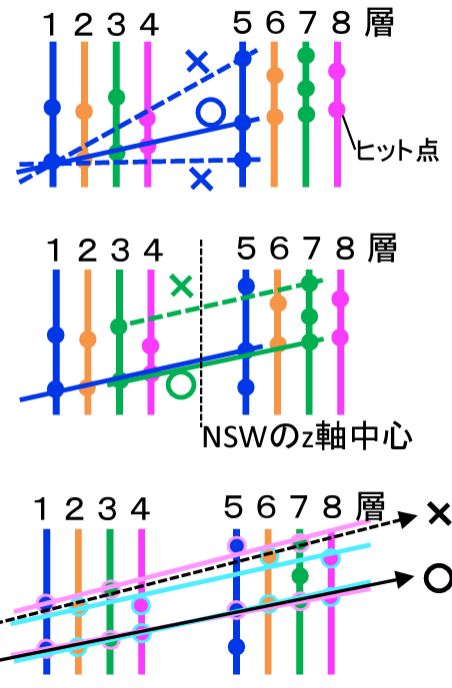
\includegraphics[clip, width=6cm]{fig/5/sTGC_hitSelectAlg.png}
  \caption{L2MuonSAにおけるsTGCヒット選択アルゴリズムの概要図\cite{article:kumaokaJPS}。}
  \label{fig:5-1}
\end{figure}

sTGCヒット選択アルゴリズムの流れを以下に示す。
\begin{enumerate}
    \item $i$層目と$i+4$層目~($i=1, 2, 3, 4$)のヒットをペア1にし、ペア1を結ぶ直線の傾きの絶対値が0.14rad以下あるいは0.6rad以上あるペア1を除外する。また切片が原点から300mm以上離れているペア1も除外する。またペア1に1つしかヒットがない場合、原点と片方のヒットでペア1を作成する。
    \item 1で残ったペア1に対して、奇数層目同士~((1層目, 5層目), (3層目, 7層目))、偶数層目同士~((2層目, 6層目), (4層目, 8層目))でペア2を作る。この際、$z$軸に垂直でNSWの中心を通る平面においてペア1の直線同士の距離が50mm以上離れているペア2は除外する。
    \item 2で作成したペア2を組み合わせて、最大8つのヒットで構成されるペア3を作成する。この時に$z$軸に垂直でNSWの中心を通る平面においてペア2の直線同士の距離が100mm以上離れているペア3は除外する。またペア2の切片の平均値の絶対値が100mm以上のペア3も除外する。
    \item ペア3の中で、以下の式で表される位置のばらつき$s$が最小の組み合わせを選択する。
    \begin{equation}
        s=\frac{1}{n-2} \sum_{i=1}^n\left(\hat{y}_i-y_i\right)^2\label{equ-5-1}
    \end{equation}
    ここで$n$は組み合わせの中にあるヒット数、$y_i$は各ヒットの$R$座標、$\hat{y}_i$は組み合わせを最小二乗法によりフィットした直線の各層の$z$座標における$R$座標である。
\end{enumerate}

上記で選ばれた最大8つのヒットを~MMのヒットと組み合わせて~SPの再構成に用いる。

\subsubsection{MMヒット選択アルゴリズム}
第2章で述べたように~MMにはストリップが底面に平行な~$X$層と$\pm15^\circ$傾けて配置された~$U$~($V$)層がある。
$X$層、$U$層、$V$層は図~\ref{fig:2-26}の順に並べられている。

sTGCと同様に~MMのヒットもクラスタリングされたヒット情報を用いて、エンドキャップ領域で定義されたロード内のヒットを選び、さらに~MMヒット選択アルゴリズムを用いて~NSWでの~SPの再構成に用いる~MMヒットを選択する。

MMヒット選択アルゴリズムの流れを以下に示す。
\begin{enumerate}
    \item $X$層(1層目, 7層目)、$X$層(2層目, 8層目)、$U$層(3層目, 5層目)、$V$層(4層目, 6層目)のヒットでペア1を作成し、ペア1を結ぶ直線の傾きの絶対値が0.1rad以下あるいは0.7rad以上あるペア1を除外する。また切片が原点から500mm以上離れているペア1も除外する。またペア1に1つしかヒットがない場合、原点と片方のヒットでペア1を作成する。また2つのペア1の切片の平均値の絶対値が200mm以上のペア2も除外する。
    \item 1で残ったペア1に対して、$X$層同士~((1層目, 7層目), (2層目, 8層目))、でペア2を作成する。この際、$z$軸に垂直でNSWの中心を通る平面においてペア1の直線同士の距離が50mm以上離れているペア2は除外する。
    \item $U$層と$V$層~((3層目, 5層目), (4層目, 6層目))でペア2を作る。ヒットの情報を用いて荷電粒子の各層における通過位置の$\phi$座標を求め、4層の$\phi$平均を取る。3層目、4層目と5層目、6層目でそれぞれ$\phi$の差を取り、どちらかで0.05rad以上の差があった場合は除外する。$\phi$の計算については後述する。
    \item 2と3で作成したペア2を組み合わせて、最大8つのヒットで構成されるペア3を作成する。また3で求めた$\phi$の情報を用いて各層の$R$座標を補正する。この補正についても後述する。補正された$R$座標~($R'$)と$z$座標を用いてペア3の部分飛跡を再構成し、\eqref{equ-5-1}式で表される位置のばらつき$s$が最小の組み合わせを選択する。
\end{enumerate}


\subsection{sTGCとMMのヒット組み合わせによるNSW部分飛跡再構成}\label{5-1-2}

\section{NSWを用いた横運動量の計算方法}\label{5-2}
NSWでの~SPから角度$\beta$を求めて、第3章で述べたように~LUTを用いて$p_T$を再構成する。
以下の図は~NSWにおける角度$\beta$の定義を表す。

\section{Run-3実データにおけるNSWを用いたL2MuonSAの性能評価}\label{5-3}

\subsection{性能評価の手法}
\subsection{性能評価}

\section{NSW部分飛跡再構成アルゴリズムの改良}\label{5-4}

\section{改良後の部分飛跡再構成アルゴリズムの性能評価}\label{5-5}